% 	Name		:: 	BDEEP template is based on the sthlm theme (Mark Hendry Olson (mark@hendryolson.com))
%	Author		:: 	Peter Christensen
%	Created		::	2016-04-12
%	Updated		::	June 18, 2015 at 08:45
%	Version		:: 	1.0
%	Email		:: 	pchrist@illinois.edu
%	Website		:: 	bdeep webiste
%
% 	License		:: 	This file may be distributed and/or modified under the
%                  	GNU Public License.
%
%	Description	::	This template makes use of the Stockholm theme from Mark Hendry Olson and includes items and files necessary for creating presentations on behalf of our group.


%-=-=-=-=-=-=-=-=-=-=-=-=-=-=-=-=-=-=-=-=-=-=-=-=
%
%        LOADING DOCUMENT
%
%-=-=-=-=-=-=-=-=-=-=-=-=-=-=-=-=-=-=-=-=-=-=-=-=

\documentclass[newPxFont]{beamer}
\usetheme{sthlm}
%\usecolortheme{sthlmv42}

%-=-=-=-=-=-=-=-=-=-=-=-=-=-=-=-=-=-=-=-=-=-=-=-=
%        LOADING PACKAGES
%-=-=-=-=-=-=-=-=-=-=-=-=-=-=-=-=-=-=-=-=-=-=-=-=
\usepackage[utf8]{inputenc}

\usepackage{chronology}

\renewcommand{\event}[3][e]{%
  \pgfmathsetlength\xstop{(#2-\theyearstart)*\unit}%
  \ifx #1e%
    \draw[fill=black,draw=none,opacity=0.5]%
      (\xstop, 0) circle (.2\unit)%
      node[opacity=1,rotate=45,right=.2\unit] {#3};%
  \else%
    \pgfmathsetlength\xstart{(#1-\theyearstart)*\unit}%
    \draw[fill=black,draw=none,opacity=0.5,rounded corners=.1\unit]%
      (\xstart,-.1\unit) rectangle%
      node[opacity=1,rotate=45,right=.2\unit] {#3} (\xstop,.1\unit);%
  \fi}%

%-=-=-=-=-=-=-=-=-=-=-=-=-=-=-=-=-=-=-=-=-=-=-=-=
%        BEAMER OPTIONS
%-=-=-=-=-=-=-=-=-=-=-=-=-=-=-=-=-=-=-=-=-=-=-=-=

\setbeameroption{show notes}

%-=-=-=-=-=-=-=-=-=-=-=-=-=-=-=-=-=-=-=-=-=-=-=-=
%
%	PRESENTATION INFORMATION
%
%-=-=-=-=-=-=-=-=-=-=-=-=-=-=-=-=-=-=-=-=-=-=-=-=

\title{Title of Presentation}
\subtitle{Subtitle of Presentation}
\date{today's date}
\author{your name}
\institute{University of Illinois}


\begin{document}

%-=-=-=-=-=-=-=-=-=-=-=-=-=-=-=-=-=-=-=-=-=-=-=-=
%
%	TITLE PAGE
%
%-=-=-=-=-=-=-=-=-=-=-=-=-=-=-=-=-=-=-=-=-=-=-=-=

\maketitle

%\begin{frame}[plain]
%	\titlepage
%\end{frame}

%-=-=-=-=-=-=-=-=-=-=-=-=-=-=-=-=-=-=-=-=-=-=-=-=
%
%	TABLE OF CONTENTS: OVERVIEW
%
%-=-=-=-=-=-=-=-=-=-=-=-=-=-=-=-=-=-=-=-=-=-=-=-=

\section*{Introduction}

%-=-=-=-=-=-=-=-=-=-=-=-=-=-=-=-=-=-=-=-=-=-=-=-=
%	FRAME:
%-=-=-=-=-=-=-=-=-=-=-=-=-=-=-=-=-=-=-=-=-=-=-=-=

\begin{frame}[c]{Introduction}

\begin{enumerate}
\item{Food security and agricultural policies often adjust the allocation of resources to achieve particular objectives -- land use, production practices, consumer behavior}   
\item{In the developing world, these adjustments are developed in very complicated settings, involve important trade-offs, and have enormous impacts}  
\item{Decision-makers often lack the ability to properly evaluate trade-offs or impact}
\end{enumerate}

\end{frame}



\section*{Overview}
\begin{frame}{Overview}
% For longer presentations use hideallsubsections option
\tableofcontents[hideallsubsections]
\end{frame}


%-=-=-=-=-=-=-=-=-=-=-=-=-=-=-=-=-=-=-=-=-=-=-=-=
%
%	SECTION: BACKGROUND
%
%-=-=-=-=-=-=-=-=-=-=-=-=-=-=-=-=-=-=-=-=-=-=-=-=

\section{Background: China's Farmland Protection Program}

%-=-=-=-=-=-=-=-=-=-=-=-=-=-=-=-=-=-=-=-=-=-=-=-=
%	FRAME:
%-=-=-=-=-=-=-=-=-=-=-=-=-=-=-=-=-=-=-=-=-=-=-=-=
\begin{frame}[c]{China Becomes a Net Grain Importer}
\begin{figure}
	\centering
	\includegraphics[width=0.65\linewidth]{Importer.png}
\end{figure}
\begin{enumerate}  
	\item{Incomes and consumption of cereal equivalents rise in post-reform period}
	\item{China undergoes the most extensive process of agricultural land conversion in the history of the world}  
\end{enumerate}  
\end{frame}

%-=-=-=-=-=-=-=-=-=-=-=-=-=-=-=-=-=-=-=-=-=-=-=-=
%	FRAME:
%-=-=-=-=-=-=-=-=-=-=-=-=-=-=-=-=-=-=-=-=-=-=-=-=
\begin{frame}[c]{Farmland Protection Policy }
	\begin{columns}
		\begin{column}{.68\linewidth}
			\begin{enumerate}   
				\item{Farmland Protection Policy (1997)}
				\begin{itemize}  
					\item{Objective: increase national self-sufficiency by halting the conversion of agricultural land}
					\item{provincial governments must ensure 'no net loss' of farmland within province}
					\item{developers can convert existing farmland and pay a fee to reclaim lands elsewehere}
				\end{itemize}  
			\end{enumerate}
		\end{column}
		\begin{column}{.3\linewidth}
			\begin{figure}
				\centering
				\includegraphics[width=0.9\linewidth]{Brown.png}
			\end{figure}
		\end{column}
	\end{columns}
\end{frame}


%-=-=-=-=-=-=-=-=-=-=-=-=-=-=-=-=-=-=-=-=-=-=-=-=
%	FRAME:
%-=-=-=-=-=-=-=-=-=-=-=-=-=-=-=-=-=-=-=-=-=-=-=-=
\begin{frame}[c]{Why do we need to evaluate the policy?}
	Farmland Protection has Become a Highly Controversial Policy	
	\begin{enumerate}   
		\item{Is this the right policy for ensuring food security?}  
		\begin{itemize}
			\item{What is the expected impact of domestic grain production on poverty/health outcomes?}
		\end{itemize}
		\item{What are the trade-offs associated with these kind of land controls?}
		\begin{itemize}
			\item{Possible distortions in/around urban land markets}
		\end{itemize}
		\item{Can we expect the policy to be effective given known corruption issues and black market land transactions?}
		\begin{itemize}
			\item{State units and collective organizations are heavily involved in illegal land conversion -- official data likely not valid}
		\end{itemize}
	\end{enumerate}	
\end{frame}

%-=-=-=-=-=-=-=-=-=-=-=-=-=-=-=-=-=-=-=-=-=-=-=-=
%
%	SECTION: UPDATES
%
%-=-=-=-=-=-=-=-=-=-=-=-=-=-=-=-=-=-=-=-=-=-=-=-=

\section{Data and Policy Evaluation}
%-=-=-=-=-=-=-=-=-=-=-=-=-=-=-=-=-=-=-=-=-=-=-=-=
%	FRAME: Images
%-=-=-=-=-=-=-=-=-=-=-=-=-=-=-=-=-=-=-=-=-=-=-=-=
\begin{frame}[c]{Measuring Land Conversion with Landsat TM}
	\begin{columns}
		\begin{column}{.6\linewidth}
			\begin{figure}
				\centering
				\includegraphics[width=0.4\linewidth]{Landsat8.jpg}
			\end{figure}
	\begin{itemize}
		\item{Observations of agricultural conversion (growth/loss) at 30X30 m2 across China}\\
		\item{3 periods: 1990-1995, 1995-2000, 2000-2005}\\
		\item{n = 10,000,000 observations X p = 6 dimensions}\\
	\end{itemize}
%			\begin{figure}
%				\centering
%				\includegraphics[width=1.2\linewidth]{Spectral.png}
%			\end{figure}
		\end{column}
		\begin{column}{.6\linewidth}
			\begin{figure}
				\centering
				\includegraphics[width=.8\linewidth]{CompareHighestResi.eps}
			\end{figure}
		\end{column}
	\end{columns}
\end{frame}


%-=-=-=-=-=-=-=-=-=-=-=-=-=-=-=-=-=-=-=-=-=-=-=-=
%	FRAME:
%-=-=-=-=-=-=-=-=-=-=-=-=-=-=-=-=-=-=-=-=-=-=-=-=
\begin{frame}{Model of Land Conversion}
	Land conversion occurs the value of land in urban use exceeds the value in agricultural use.
	\begin{equation}{\label{eq1}}
	V_{i,t}^{u}-(\sum\limits_{T=0}^{\infty}V_{i,t+T}^{a})\delta^{T}-C_{t}^{a}>0   
	\end{equation}
	Farmland protection adds an additional cost ($C^{\tau}$), which should affect the rate at which agricultural land is developed.
	\begin{equation}{\label{eq2}}
	L_{it}^{u}=f(V_{it}^{a},C_{it}^{a},C^{\tau})
	\end{equation}
\end{frame}

%-=-=-=-=-=-=-=-=-=-=-=-=-=-=-=-=-=-=-=-=-=-=-=-=
%	FRAME: Images
%-=-=-=-=-=-=-=-=-=-=-=-=-=-=-=-=-=-=-=-=-=-=-=-=

\begin{frame}{Images with Copyright}
	I estimate the effect of the protection policy by comparing conversion rates in provinces where the policy binds to provinces where it does not.
	\begin{equation}{\label{eq2}}
		\tau_{ATT(\frac{da}{du})}=[\frac{dL^{a}}{dL^{u}}_{it}(1)-\frac{dL^{a}}{dL^{u}}_{it}(0)]
	\end{equation}
	\begin{figure}
		\centering
		\includegraphics[width=0.6\linewidth, trim=0 0 0 400, clip]{CompareHiRes_Guangzhou.eps}
	\end{figure}
\end{frame}

%-=-=-=-=-=-=-=-=-=-=-=-=-=-=-=-=-=-=-=-=-=-=-=-=
%	FRAME:
%-=-=-=-=-=-=-=-=-=-=-=-=-=-=-=-=-=-=-=-=-=-=-=-=


\begin{frame}[c]{Policy Timeline}
	\vspace{-1cm}
	\begin{center}\begin{chronology}[5]{1988}{2005}{0.85\textwidth}
			\event[\decimaldate{1}{1}{1990}]{\decimaldate{1}{11}{1994}}{\cRed{Period 1}}
			\event[\decimaldate{1}{3}{1995}]{\decimaldate{1}{11}{1999}}{ 1997 - No Net Loss Regulation}
			\event[\decimaldate{1}{3}{2000}]{\decimaldate{1}{1}{2005}}{\cRed{Period 2}}
		\end{chronology}
	\end{center}
	
\end{frame}


%-=-=-=-=-=-=-=-=-=-=-=-=-=-=-=-=-=-=-=-=-=-=-=-=
%
%	SECTION: STRUCTURE
%
%-=-=-=-=-=-=-=-=-=-=-=-=-=-=-=-=-=-=-=-=-=-=-=-=
\section{Primary Findings}

%-=-=-=-=-=-=-=-=-=-=-=-=-=-=-=-=-=-=-=-=-=-=-=-=
%	FRAME:
%-=-=-=-=-=-=-=-=-=-=-=-=-=-=-=-=-=-=-=-=-=-=-=-=

\begin{frame}[c]{Results}
	Primary Findings	
	\begin{enumerate}   
		\item{Was the policy effective in reducing farmland conversion?}  
		\begin{itemize}
			\item{Overall, regulation had a huge impact on China's land market}
			\item{Province-level rates of farmland conversion fell by 39-56\% relative to the policy counterfactual}
			\item{Evidence of non-compliance (full compliance = 100\%)}
		\end{itemize}
	\end{enumerate}	
\end{frame}

%-=-=-=-=-=-=-=-=-=-=-=-=-=-=-=-=-=-=-=-=-=-=-=-=
%	FRAME:
%-=-=-=-=-=-=-=-=-=-=-=-=-=-=-=-=-=-=-=-=-=-=-=-=

\begin{frame}[c]{Results}
	Primary Findings	
	\begin{enumerate}   
		\item{What are the trade-offs and distortions associated with these kind of land controls?}
		\begin{itemize}
			\item{On average, the policy reduced urban expansion by 11\% relative to the counterfactual.}
			\item{The magnitude is much higher in cities where pre-policy conversion rates were higher (up to 50\%).}
			\item{What is the cost in terms of forgone productivity?  We're working on that right now...}
			\item{Urban distortions: policy displaced 1\% of land that would have occurred within 10km of a city center to outside (effect is 6.7\% in high conversion cities)}
		\end{itemize}
	\end{enumerate}	
\end{frame}

%-=-=-=-=-=-=-=-=-=-=-=-=-=-=-=-=-=-=-=-=-=-=-=-=
%
%	SECTION: ADDITIONAL FEATURES
%
%-=-=-=-=-=-=-=-=-=-=-=-=-=-=-=-=-=-=-=-=-=-=-=-=
\section{Conclusions and Insights}

%-=-=-=-=-=-=-=-=-=-=-=-=-=-=-=-=-=-=-=-=-=-=-=-=
%	FRAME: Concluding Remarks
%-=-=-=-=-=-=-=-=-=-=-=-=-=-=-=-=-=-=-=-=-=-=-=-=

\begin{frame}[c]{Conclusions}
	Primary Conclusions
	\begin{enumerate}   
		\item{Land controls are probably not a sensible regulatory tool for food security}  
		\begin{itemize}
			\item{Possible deleterious impact on rural incomes}
			\item{Very high societal costs, particularly in urbanizing regions}
			\item{Range of unintended consequences}
		\end{itemize}
		\item{New Data for Policy Evaluation}
		\begin{itemize}
			\item{We can monitor the effects of very large programs (ex. national policy, administered at the provincial level)}
			\item{It is possible to combine these data with (geo-referenced) measures of household income, poverty/health outcomes, consumption behavior to understand nuanced impacts at very large scales}
			\item{Key -- valid statistical model (identification)}
		\end{itemize}
	\end{enumerate}	
\end{frame}

%-=-=-=-=-=-=-=-=-=-=-=-=-=-=-=-=-=-=-=-=-=-=-=-=
%
%	SECTION: Conclusion
%
%-=-=-=-=-=-=-=-=-=-=-=-=-=-=-=-=-=-=-=-=-=-=-=-=

\begin{frame}{Links to More}
	
You can find this working paper and my other publications at \url{www.peterchristensen.net}.\\
\vspace{1em}
If you are interested in learning about the technology that we are building to support our economics and policy research, please come find us on the 3rd floor of the National Center for Supercomputing Applications (NCSA).\\
\vspace{1em}	
Please send questions and comments to: pchrist@illinois.edu
\end{frame}

\end{document}